%!Mode:: "TeX:UTF-8"
\documentclass[a4paper,11pt,UTF8]{ctexart}

\usepackage{indentfirst} %缩进
\usepackage{xeCJK}    %使用系统字体
\usepackage{fancyhdr} %自定义页眉页脚
\pagestyle{empty}                   %不设置页眉页脚
\usepackage{amsmath, amsthm, amssymb, amsfonts} %数学公式
\usepackage[a4paper,left=3cm,right=3cm,top=3cm,bottom=3cm]{geometry}
%\usepackage[tmargin=1in,bmargin=1in,lmargin=1.25in,rmargin=1.25in]{geometry}.
\usepackage{booktabs} %插入表格
\usepackage[section]{placeins} %避免浮动
\usepackage{listings} %插入代码
\usepackage{ctex}     %中文宏包
\usepackage[svgnames, table]{xcolor} %彩色表格
\usepackage{algorithm}          %伪代码
\usepackage{algorithmicx}
\usepackage{algpseudocode}
\usepackage{algorithm,algpseudocode,float}
\usepackage{lipsum}
\usepackage{enumitem}           %调整列举环境
\usepackage{url}
\usepackage{fontspec,xunicode}
\defaultfontfeatures{Mapping=tex-text} %如果没有它,会有一些 tex 特殊字符无法正常使用,比如连字符。

\usepackage{graphicx}
\graphicspath{{imgs/}}

%%%%%%%%%%%%%%%%%%%%%%%%%%%%%%%%%%%%%%%%%%%%%%%%%%%%%%%%%%%%%%%%
% 缩进及行间距
%%%%%%%%%%%%%%%%%%%%%%%%%%%%%%%%%%%%%%%%%%%%%%%%%%%%%%%%%%%%%%%%
\setlength{\parindent}{22pt} %重新定义缩进长度
\setlength{\baselineskip}{20pt}  %定义行间距
%\renewcommand{\baselinestretch}{1.1} %定义行间距

%%%%%%%%%%%%%%%%%%%%%%%%%%%%%%%%%%%%%%%%%%%%%%%%%%%%%%%%%%%%%%%%
% 列表设置
%%%%%%%%%%%%%%%%%%%%%%%%%%%%%%%%%%%%%%%%%%%%%%%%%%%%%%%%%%%%%%%%
\setenumerate{fullwidth,itemindent=\parindent,listparindent=\parindent,itemsep=0ex,partopsep=0pt,parsep=0ex}
\setenumerate[2]{label=\alph*),leftmargin=1.5em}  %二级item设置
\setitemize{itemindent=38pt,leftmargin=0pt,itemsep=-0.4ex,listparindent=26pt,partopsep=0pt,parsep=0.5ex,topsep=-0.25ex}
\setdescription{itemindent=38pt,leftmargin=0pt,itemsep=-0.4ex,listparindent=26pt,partopsep=0pt,parsep=0.5ex,topsep=-0.25ex}

%%%%%%%%%%%%%%%%%%%%%%%%%%%%%%%%%%%%%%%%%%%%%%%%%%%%%%%%%%%%%%%%
% 图的标题行间距设置
%%%%%%%%%%%%%%%%%%%%%%%%%%%%%%%%%%%%%%%%%%%%%%%%%%%%%%%%%%%%%%%%
\newcommand{\bottomcaption}{%
\setlength{\abovecaptionskip}{6pt}%
\setlength{\belowcaptionskip}{6pt}%
\caption}


%%%%%%%%%%%%%%%%%%%%%%%%%%%%%%%%%%%%%%%%%%%%%%%%%%%%%%%%%%%%%%%%
% 字体定义
%%%%%%%%%%%%%%%%%%%%%%%%%%%%%%%%%%%%%%%%%%%%%%%%%%%%%%%%%%%%%%%%
\setmainfont{Times New Roman}  %默认英文字体.serif是有衬线字体sans serif无衬线字体
\setmonofont{Consolas}
\setCJKmainfont[ItalicFont={楷体}, BoldFont={黑体}]{宋体}%衬线字体 缺省中文字体为
\setCJKsansfont{黑体}
\punctstyle{hangmobanjiao}
%-----------------------xeCJK下设置中文字体------------------------------%
\setCJKfamilyfont{song}{SimSun}                             %宋体 song
\newcommand{\song}{\CJKfamily{song}}
\setCJKfamilyfont{fs}{FangSong}                      %仿宋  fs
\newcommand{\fs}{\CJKfamily{fs}}
\setCJKfamilyfont{ktgb}{KaiTi}                      %楷体2312 ktgb
\newcommand{\ktgb}{\CJKfamily{ktgb}}
\setCJKfamilyfont{yh}{Microsoft YaHei}                    %微软雅黑 yh
\newcommand{\yh}{\CJKfamily{yh}}
\setCJKfamilyfont{hei}{SimHei}                              %黑体  hei
\newcommand{\hei}{\CJKfamily{hei}}
\setCJKfamilyfont{hwxk}{STXingkai}                                %华文行楷  hwxk
\newcommand{\hwxk}{\CJKfamily{hwxk}}
%------------------------------设置字体大小------------------------%
\newcommand{\shiyanbaogao}{\fontsize{36pt}{\baselineskip}\selectfont}
\newcommand{\chuhao}{\fontsize{42pt}{\baselineskip}\selectfont}     %初号
\newcommand{\xiaochuhao}{\fontsize{36pt}{\baselineskip}\selectfont} %小初号
\newcommand{\yihao}{\fontsize{28pt}{\baselineskip}\selectfont}      %一号
\newcommand{\erhao}{\fontsize{21pt}{\baselineskip}\selectfont}      %二号
\newcommand{\xiaoerhao}{\fontsize{18pt}{\baselineskip}\selectfont}  %小二号
\newcommand{\sanhao}{\fontsize{15.75pt}{\baselineskip}\selectfont}  %三号
\newcommand{\sihao}{\fontsize{14pt}{\baselineskip}\selectfont}       %四号
\newcommand{\xiaosihao}{\fontsize{12pt}{\baselineskip}\selectfont}  %小四号
\newcommand{\wuhao}{\fontsize{10.5pt}{\baselineskip}\selectfont}    %五号
\newcommand{\xiaowuhao}{\fontsize{9pt}{\baselineskip}\selectfont}   %小五号
\newcommand{\liuhao}{\fontsize{7.875pt}{\baselineskip}\selectfont}  %六号
\newcommand{\qihao}{\fontsize{5.25pt}{\baselineskip}\selectfont}    %七号

%%%%%%%%%%%%%%%%%%%%%%%%%%%%%%%%%%%%%%%%%%%%%%%%%%%%%%%%%%%%%%%%
% 图题字体大小相同
%%%%%%%%%%%%%%%%%%%%%%%%%%%%%%%%%%%%%%%%%%%%%%%%%%%%%%%%%%%%%%%%
\usepackage{caption}
\captionsetup{font={footnotesize}}   % footnotesize = 9pt
\captionsetup[lstlisting]{font={footnotesize}}

%%%%%%%%%%%%%%%%%%%%%%%%%%%%%%%%%%%%%%%%%%%%%%%%%%%%%%%%%%%%%%%%
% 重定义枚举编号为 1),2)...
%%%%%%%%%%%%%%%%%%%%%%%%%%%%%%%%%%%%%%%%%%%%%%%%%%%%%%%%%%%%%%%%
\renewcommand{\labelenumi}{\theenumi)}

%%%%%%%%%%%%%%%%%%%%%%%%%%%%%%%%%%%%%%%%%%%%%%%%%%%%%%%%%%%%%%%%
% 标题名称中文化
%%%%%%%%%%%%%%%%%%%%%%%%%%%%%%%%%%%%%%%%%%%%%%%%%%%%%%%%%%%%%%%%
\renewcommand\figurename{\hei 图}
\renewcommand\tablename{\hei 表}
\renewcommand\lstlistingname{\hei 代码}
\renewcommand{\algorithmicrequire}{\textbf{输入:}}
\renewcommand{\algorithmicensure}{\textbf{输出:}}
\newtheorem{define}{定义}

%%%%%%%%%%%%%%%%%%%%%%%%%%%%%%%%%%%%%%%%%%%%%%%%%%%%%%%%%%%%%%%%
% 代码设置
%%%%%%%%%%%%%%%%%%%%%%%%%%%%%%%%%%%%%%%%%%%%%%%%%%%%%%%%%%%%%%%%
\lstset{
 columns=fixed,
 numbers=left,                                        % 在左侧显示行号
 numberstyle=\tiny\color{gray},                       % 设定行号格式
 frame=single,                                        % 单线背景边框
 breaklines=true,                                     % 设定LaTeX对过长的代码行进行自动换行
 keywordstyle=\color[RGB]{40,40,255},                 % 设定关键字颜色
 numberstyle=\footnotesize\color{darkgray},
 commentstyle=\it\color[RGB]{0,96,96},                % 设置代码注释的格式
 stringstyle=\rmfamily\slshape\color[RGB]{128,0,0},   % 设置字符串格式
 showstringspaces=false,                              % 不显示字符串中的空格
 language=java,                                        % 设置语言
 basicstyle=\linespread{1.0}\xiaowuhao\ttfamily,                      % 字体字号
 %lineskip=10pt,
 %baselinestretch=1,
}

%%%%%%%%%%%%%%%%%%%%%%%%%%%%%%%%%%%%%%%%%%%%%%%%%%%%%%%%%%%%%%%%
% 伪代码分页
%%%%%%%%%%%%%%%%%%%%%%%%%%%%%%%%%%%%%%%%%%%%%%%%%%%%%%%%%%%%%%%%
\makeatletter
\renewcommand{\ALG@name}{算法}
\newenvironment{breakablealgorithm}
  {% \begin{breakablealgorithm}
   \begin{center}
     \refstepcounter{algorithm}% New algorithm
     \hrule height.8pt depth0pt \kern2pt% \@fs@pre for \@fs@ruled
     \renewcommand{\caption}[2][\relax]{% Make a new \caption
       {\raggedright\textbf{\ALG@name~\thealgorithm} ##2\par}%
       \ifx\relax##1\relax % #1 is \relax
         \addcontentsline{loa}{algorithm}{\protect\numberline{\thealgorithm}##2}%
       \else % #1 is not \relax
         \addcontentsline{loa}{algorithm}{\protect\numberline{\thealgorithm}##1}%
       \fi
       \kern2pt\hrule\kern2pt
     }
  }{% \end{breakablealgorithm}
     \kern2pt\hrule\relax% \@fs@post for \@fs@ruled
   \end{center}
  }
\makeatother

% =============================================
% Part 1 Edit the info
% =============================================

\newcommand{\major}{物理学院}
\newcommand{\name}{黄阅迅,李秋阳}
\newcommand{\stuid}{PB18020631,PB18020567}
\newcommand{\group}{20}
\newcommand{\newdate}{\today}


\newcommand{\course}{电子线路实验(1)}
\newcommand{\newtitle}{数据编码器和译码器}

% =============================================
% Part 1 Main document
% =============================================
\begin{document}
\thispagestyle{empty}
\begin{figure}[h]
  \begin{minipage}{0.6\linewidth}
    \centerline{
\includegraphics[width=\linewidth]{logo.png}}
  \end{minipage}
  \hfill
  \begin{minipage}{.4\linewidth}
    \raggedleft
    \begin{tabular*}{.8\linewidth}{ll}
      学院: & \underline\major   \\
      姓名: & \underline\name    \\
      学号: & \underline\stuid   \\
      组号:  & \underline\group   \\
      日期: & \underline\newdate \\
    \end{tabular*}
  \end{minipage}
\end{figure}

\begin{table}[!htbp]
  \centering
  \begin{tabular*}{\linewidth}{llllll}
    课程名称:  \underline\course   \qquad\qquad 实验题目:  \underline\newtitle  
  \end{tabular*}
\end{table}

% =============================================
% Part 2 Main document
% =============================================

\section{实验目的}

请参看预习报告。

\section{实验原理}

请参看预习报告。

\section{实验内容与步骤}
\subsection{实验一:验证编码器74LS148和译码器74LS138的逻辑功能}
	\par 74LS148 是8线-3线编码器,74LS138 是3线-8线译码器。所以将二者3线端口直接相连,用 LED 灯的亮灭来检测高低电平,就可以看到编码和译码的全过程。由此得到电路图:
	\begin{figure}[H]
	 \centering
	 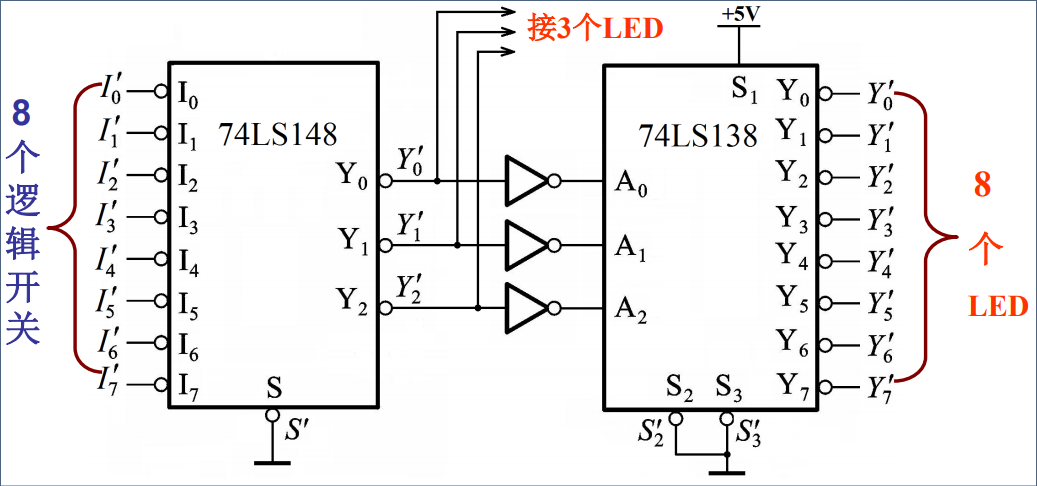
\includegraphics[width=0.5\linewidth]{Exp01}
	 \caption{实验一电路图}
	 \label{fig:exp01}
	\end{figure}
	\par 由此写出 74LS148 和 74LS138 的真值表。
	\par 真值表为:
	\begin{table}[H]
	\centering
	\resizebox{\textwidth}{!}{
	 \begin{tabular}{|cccccccc|ccc|ccc|cccccccc|}
	  \hline
	  \multicolumn{11}{|c|}{74LS148} &
	  \multicolumn{11}{c|}{74LS138} \\
	  \hline
	  $I_0'$&$I_1'$&$I_2'$&$I_3'$&$I_4'$&$I_5'$&$I_6'$&$I_6'$
	  &$Y_2'$&$Y_1'$&$Y_0'$
	  &$A_2$&$A_1$&$A_0$
	  &$Y_0'$&$Y_1'$&$Y_2'$&$Y_3'$&$Y_4'$&$Y_5'$&$Y_6'$&$Y_6'$
	  \\\hline
	  1&1&1&1&1&1&1&1 &1&1&1 &0&0&0 &0&1&1&1&1&1&1&1
	  \\\hline
	  0&1&1&1&1&1&1&1 &1&1&1 &0&0&0 &0&1&1&1&1&1&1&1
	  \\\hline
		X&0&1&1&1&1&1&1 &1&1&0 &0&0&1 &1&0&1&1&1&1&1&1
		\\\hline
		X&X&0&1&1&1&1&1 &1&0&1 &0&1&0 &1&1&0&1&1&1&1&1
		\\\hline
		X&X&X&0&1&1&1&1 &1&0&0 &0&1&1 &1&1&1&0&1&1&1&1
		\\\hline
		X&X&X&X&0&1&1&1 &0&1&1 &1&0&0 &1&1&1&1&0&1&1&1
		\\\hline
		X&X&X&X&X&0&1&1 &0&1&0 &1&0&1 &1&1&1&1&1&0&1&1
		\\\hline
		X&X&X&X&X&X&0&1 &0&0&1 &1&1&0 &1&1&1&1&1&1&0&1
		\\\hline
		X&X&X&X&X&X&X&0 &0&0&0 &1&1&1 &1&1&1&1&1&1&1&0
		\\\hline
	 \end{tabular}
	 }
	 \caption{实验一真值表}
	\end{table}
	
\subsection{实验二:用两片74LS138扩展为一个4线–16线译码器}
	\par 因为需要 16 位输出,所以需要两片 74LS138。
	\par 将输入设为 $D_0,~D_1,~D_2,~D_3$,设 $D_3$ 为最高位(MSB),那么低三位可以用一个译码器去处理,设为译码器1。另一个译码器设为译码器2。
	\par 如果 $D_3=0$,那么该位等于不存在,输出的唯一低电平一定在译码器1上。所以只需要保证此时译码器2输出全为1(无效)。
	\par 如果 $D_3=1$,那么该位提供的权重为 $8_D$,此时输出的唯一低电平一定在译码器2上。而且可以发现,如果输出相差8位,那么正好是处在不同编译器的相同位置上。所以,对于两个译码器来说,3位输入线接法是一样的。只需要保证 $D_3=0$ 时,只有编码器1工作;$D_3=1$ 时,只有编码器2工作。因此可以给出如下的电路图:
	\begin{figure}[H]
	 \centering
	 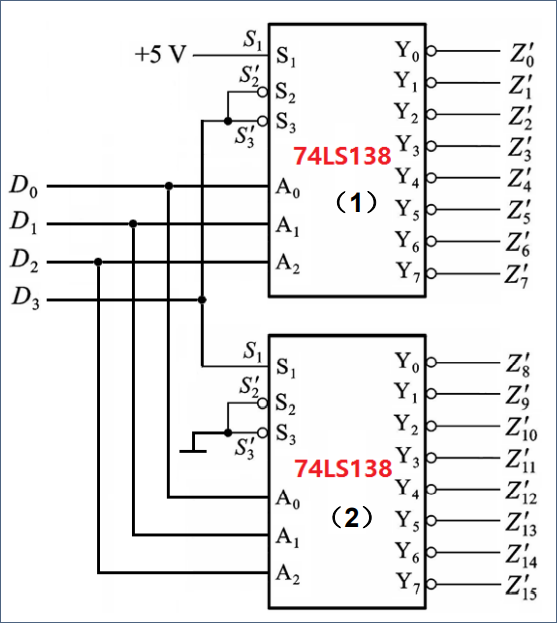
\includegraphics[width=0.5\linewidth]{Exp02}
	 \caption{实验二电路图}
	 \label{fig:exp02}
	\end{figure}
	\par 由此写出整个4线-16线译码器的真值表。
	\par 真值表为:
	\begin{table}[H]
	 \centering
	 \resizebox{\textwidth}{!}{
	 \begin{tabular}{|cccc|cccccccccccccccc|}
	  \hline
	 	$D_3$&$D_2$&$D_1$&$D_0$
	 	&$Z_0'$&$Z_1'$&$Z_2'$&$Z_3'$&$Z_4'$&$Z_5'$&$Z_6'$&$Z_7'$
	 	&$Z_8'$&$Z_9'$&$Z_{10}'$&$Z_{11}'$&$Z_{12}'$&$Z_{13}'$
	 	&$Z_{14}'$&$Z_{15}'$
	 	\\\hline
	 	0&0&0&0 &0&1&1&1 &1&1&1&1 &1&1&1&1 &1&1&1&1
	 	\\\hline
	 	0&0&0&1 &1&0&1&1 &1&1&1&1 &1&1&1&1 &1&1&1&1
	 	\\\hline
	 	0&0&1&0 &1&1&0&1 &1&1&1&1 &1&1&1&1 &1&1&1&1
	 	\\\hline
	 	0&0&1&1 &1&1&1&0 &1&1&1&1 &1&1&1&1 &1&1&1&1
	 	\\\hline
	 	0&1&0&0 &1&1&1&1 &0&1&1&1 &1&1&1&1 &1&1&1&1
	 	\\\hline
	 	0&1&0&1 &1&1&1&1 &1&0&1&1 &1&1&1&1 &1&1&1&1
	 	\\\hline
	 	0&1&1&0 &1&1&1&1 &1&1&0&1 &1&1&1&1 &1&1&1&1
	 	\\\hline
	 	0&1&1&1 &1&1&1&1 &1&1&1&0 &1&1&1&1 &1&1&1&1
	 	\\\hline
	 	1&0&0&0 &1&1&1&1 &1&1&1&1 &0&1&1&1 &1&1&1&1
	 	\\\hline
	 	1&0&0&1 &1&1&1&1 &1&1&1&1 &1&0&1&1 &1&1&1&1
	 	\\\hline
	 	1&0&1&0 &1&1&1&1 &1&1&1&1 &1&1&0&1 &1&1&1&1
	 	\\\hline
	 	1&0&1&1 &1&1&1&1 &1&1&1&1 &1&1&1&0 &1&1&1&1
	 	\\\hline
	 	1&1&0&0 &1&1&1&1 &1&1&1&1 &1&1&1&1 &0&1&1&1
	 	\\\hline
	 	1&1&0&1 &1&1&1&1 &1&1&1&1 &1&1&1&1 &1&0&1&1
	 	\\\hline
	 	1&1&1&0 &1&1&1&1 &1&1&1&1 &1&1&1&1 &1&1&0&1
	 	\\\hline
	 	1&1&1&1 &1&1&1&1 &1&1&1&1 &1&1&1&1 &1&1&1&0
	 	\\\hline
	 \end{tabular}
	 }
	 \caption{实验二真值表}
	\end{table}

\subsection{实验三:用74LS138和74LS20双与非门设计控制电路}
	\par {\kaishu 某工厂有三个车间 $A,~B,~C$ 和一个自备发电站,站内有两台发电机 $M,~N$ 发电机 $N$ 的发电能力是 $M$ 的两倍。如果一个车间开工,启动 $M$ 就可以满足要求;如果两个车间开工,启动 $N$ 就可以满足要求;如果三个车间均开工,同时启动 $M$ 和 $N$ 才能满足要求。设计控制发电机的逻辑电路。
	}
	\par 逻辑表达式为:
	\[ M=A'B'C+A'BC'+AB'C'+ABC=\sum m(0,1,2,4,7)
	=(m_1'm_2'm_4'm_7')'\]
	\[ N=A'BC+AB'C+ABC'+ABC=\sum m(3,5,6,7)
	=(m_3'm_5'm_6'm_7')'\]
	\par 将 $A,~B,~C$接在 74LS138 的输入端,接下来只要将输出进行逻辑操作就可以了。设计电路图为:
	\begin{figure}[H]
	 \centering
	 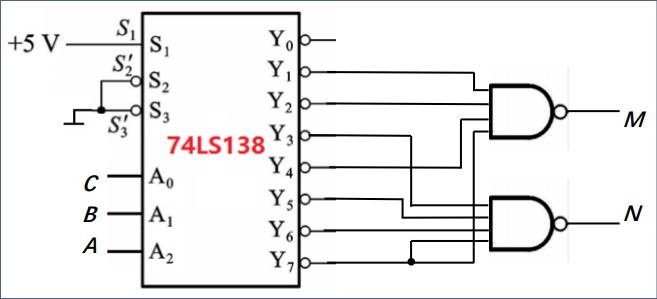
\includegraphics[width=0.5\linewidth]{Exp03}
	 \caption{实验三电路图}
	 \label{fig:exp03}
	\end{figure}
	\par 由此写出输入与输出的真值表。
	真值表为:
	\begin{table}[H]
	 \centering
	 \begin{tabular}{|ccc|cc|}\hline
	  $A$&$B$&$C$ &$M$&$N$
	  \\\hline
	  0&0&0 &0&0
	  \\\hline
	  0&0&1 &1&0
	  \\\hline
	  0&1&0 &1&0
	  \\\hline
	  0&1&1 &0&1
	  \\\hline
	  1&0&0 &1&0
	  \\\hline
	  1&0&1 &0&1
	  \\\hline
	  1&1&0 &0&1
	  \\\hline
	  1&1&1 &1&1
	  \\\hline
	 \end{tabular}
	 \caption{实验三真值表}
	\end{table}

\subsection{实验四:用74LS138和74LS20双与非门设计多输出函数}
	\par {\kaishu 用74LS138和74LS20双与非门设计下面的多输出函数:
	\begin{align*}
	 &F_1=\sum m(0,4)\\
	 &F_2=\sum m(1,2,3,5,6,7)\\
	\end{align*}
	画出逻辑电路图并搭建电路。
	}
	\par 逻辑表达式化简为:
	\[ F_1=\sum m(0,4)=m_0+m_4=(m_0'm_4')' \]
	\[ F_2=\sum m(1,2,3,5,6,7)=F_1' \]
	\par 将 $A_0,~A_1,~A_2$ 接在 74LS138 的输入端,接下来只要将输出进行逻辑操作就可以了。设计电路图为:
	\begin{figure}[H]
	 \centering
	 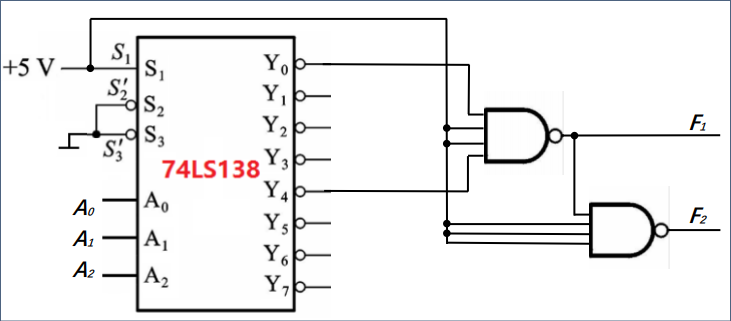
\includegraphics[width=0.5\linewidth]{Exp04}
	 \caption{实验四电路图}
	 \label{fig:exp04}
	\end{figure}
	\par 由此写出输入与输出的真值表。
	真值表为:
	\begin{table}[H]
	 \centering
	 \begin{tabular}{|ccc|cc|}\hline
	  $A_2$&$A_1$&$A_0$ &$F_1$&$F_2$
	  \\\hline
	  0&0&0 &1&0
	  \\\hline
	  0&0&1 &0&1
	  \\\hline
	  0&1&0 &0&1
	  \\\hline
	  0&1&1 &0&1
	  \\\hline
	  1&0&0 &1&0
	  \\\hline
	  1&0&1 &0&1
	  \\\hline
	  1&1&0 &0&1
	  \\\hline
	  1&1&1 &0&1
	  \\\hline
	 \end{tabular}
	 \caption{实验四真值表}
	\end{table}
	
\subsection{实验五:观察4511控制的LED}
	\par 将实验箱上4个逻辑开关的输出接到1组显示译码器 4511 的$A,~B,~C,~D$ 输入口,接上+5V显示器的电源,然后拨动开关(0000-1111),观察并记录 LED 数码管显示的对应数字,判断译码显示是否正常。
	\par 再将实验箱上的4组拨码开关的输出 $A_i,~B_i,~C_i,~D_i$ 分别接到4组显示译码器 4511 的对应输入口,按动四个数码的“+”“-” 键,观察拨码盘上的四位数与 LED 数码管显示的对应数字是否一致,译码显示是否正常。
	\par 4511 的功能表为:
	\begin{table}[H]
	 \centering
	 \begin{tabular}{|cccc|c|cccc|c|}\hline
	  \multicolumn{4}{|c|}{In} & Out
	  &\multicolumn{4}{c|}{In} &Out
	  \\\hline
	  $D$&$C$&$B$&$A$ &Type
	  &$D$&$C$&$B$&$A$ &Type
	  \\\hline
	  0&0&0&0&
	  \begin{minipage}{0.1\textwidth}
	   \centering
	   
\includegraphics[height=0.5cm]{Digit0}
	  \end{minipage}
	  &1&0&0&0&
	  \begin{minipage}{0.1\textwidth}
	   \centering
	   
\includegraphics[height=0.5cm]{Digit8}
	  \end{minipage}
	  \\\hline
	  0&0&0&1&
	  \begin{minipage}{0.1\textwidth}
	   \centering
	   
\includegraphics[height=0.5cm]{Digit1}
	  \end{minipage}
	  &1&0&0&1&
	  \begin{minipage}{0.1\textwidth}
	   \centering
	   
\includegraphics[height=0.5cm]{Digit9}
	  \end{minipage}
	  \\\hline
	  0&0&1&0&
	  \begin{minipage}{0.1\textwidth}
	   \centering
	   
\includegraphics[height=0.5cm]{Digit2}
	  \end{minipage}
	  &1&0&1&0&	\textbackslash
	  \\\hline
	  0&0&1&1&
	  \begin{minipage}{0.1\textwidth}
	   \centering
	   
\includegraphics[height=0.5cm]{Digit3}
	  \end{minipage}
	  &1&0&1&1&	\textbackslash
	  \\\hline
	  0&1&0&0&
	  \begin{minipage}{0.1\textwidth}
	   \centering
	   
\includegraphics[height=0.5cm]{Digit4}
	  \end{minipage}
	  &1&1&0&0&	\textbackslash
	  \\\hline
	  0&1&0&1&
	  \begin{minipage}{0.1\textwidth}
	   \centering
	   
\includegraphics[height=0.5cm]{Digit5}
	  \end{minipage}
	  &1&1&0&1&	\textbackslash
	  \\\hline
	  0&1&1&0&
	  \begin{minipage}{0.1\textwidth}
	   \centering
	   
\includegraphics[height=0.5cm]{Digit6}
	  \end{minipage}
	  &1&1&1&0&	\textbackslash
	  \\\hline
	  0&1&1&1&
	  \begin{minipage}{0.1\textwidth}
	   \centering
	   
\includegraphics[height=0.5cm]{Digit7}
	  \end{minipage}
	  &1&1&1&1&	\textbackslash
	  \\\hline
	 \end{tabular}
	 \caption{实验五功能表}
	\end{table}
	\par 将拨码开关与译码器相连接,变换拨码开关的数字。经过实验,发现 LED 数码管显示的数字与拨码开关拨码盘的数字完全一致。
	
\section{实验总结}
	\par 本次实验,我们使用了一些数字电路中常用的编码译码芯片。编码是将输入的一位信号(只有一位有效)转换成紧凑的 8421BCD 码;而译码是其反过程。
	\par 编码可以减少走线的数目,从而节省资源;而译码可以产生便于逻辑操作的最小项表达式(不过是低电平有效),从而可以构建出任意与输入位数一致的逻辑表达式。
	\par 生活中有很多地方用七段 LED 数码管来显示数字。对于仅仅显示数字的设备而言,数码管只有七段(有时候用到小数点,是八段),易于控制。但是尽管如此,因为需要对照着数字显示图样来确定各位的高低,使用起来还不够方便。而 4511 作为专用于数码管的译码器,可以将输入的 8421BCD 码译码成控制显示该数字的信号。这样输出的数字就与输入的 8421BCD 码简单地对应起来了,使用方便。
\section{实验思考题}
\subsection{题目一}
用两片74LS138和必要的门电路实现以下多输出函数,画出电路图。
\begin{equation}
  \begin{aligned}
    Y_1&=A'BC'D'+A'B'C'D+AB'C'D'+ABCD'\\
    Y_2&=BC
  \end{aligned}
\end{equation}

答:为设计此电路,首先需要四个输入,因此先用两片74LS138搭成4-16线译码器再进行操作。
然后进行字母指派如下(注意这里为了方便,所以可能与惯例不太一样):
\begin{equation}
  A\rightarrow D_3,B\rightarrow D_2,C\rightarrow D_1,D\rightarrow D_0
\end{equation}
于是,写出最小项表达式并化简成与非形式如下(为了不与电路图混淆,所以Y改成了F):
\begin{equation}
  \begin{aligned}
    F_1&=0100+0001+1000+1110=m_4+m_1+m_8+m_{14}=(Y_4'Y_1'Y_8'Y_{14}')'\\
    F_2&=(A+A')BC(D+D')=ABCD+A'BCD+ABCD'+A'BCD'\\
       &=1111+0111+1110+0110=m_{15}+m_7+m_{14}+m_6=(Y_{15}'Y_7'Y_{14}'Y_6')'
  \end{aligned}
\end{equation}
因此,设计的电路图如图 \ref{fig:pb1}所示。

\begin{figure}[H]
  \centering
  \fbox{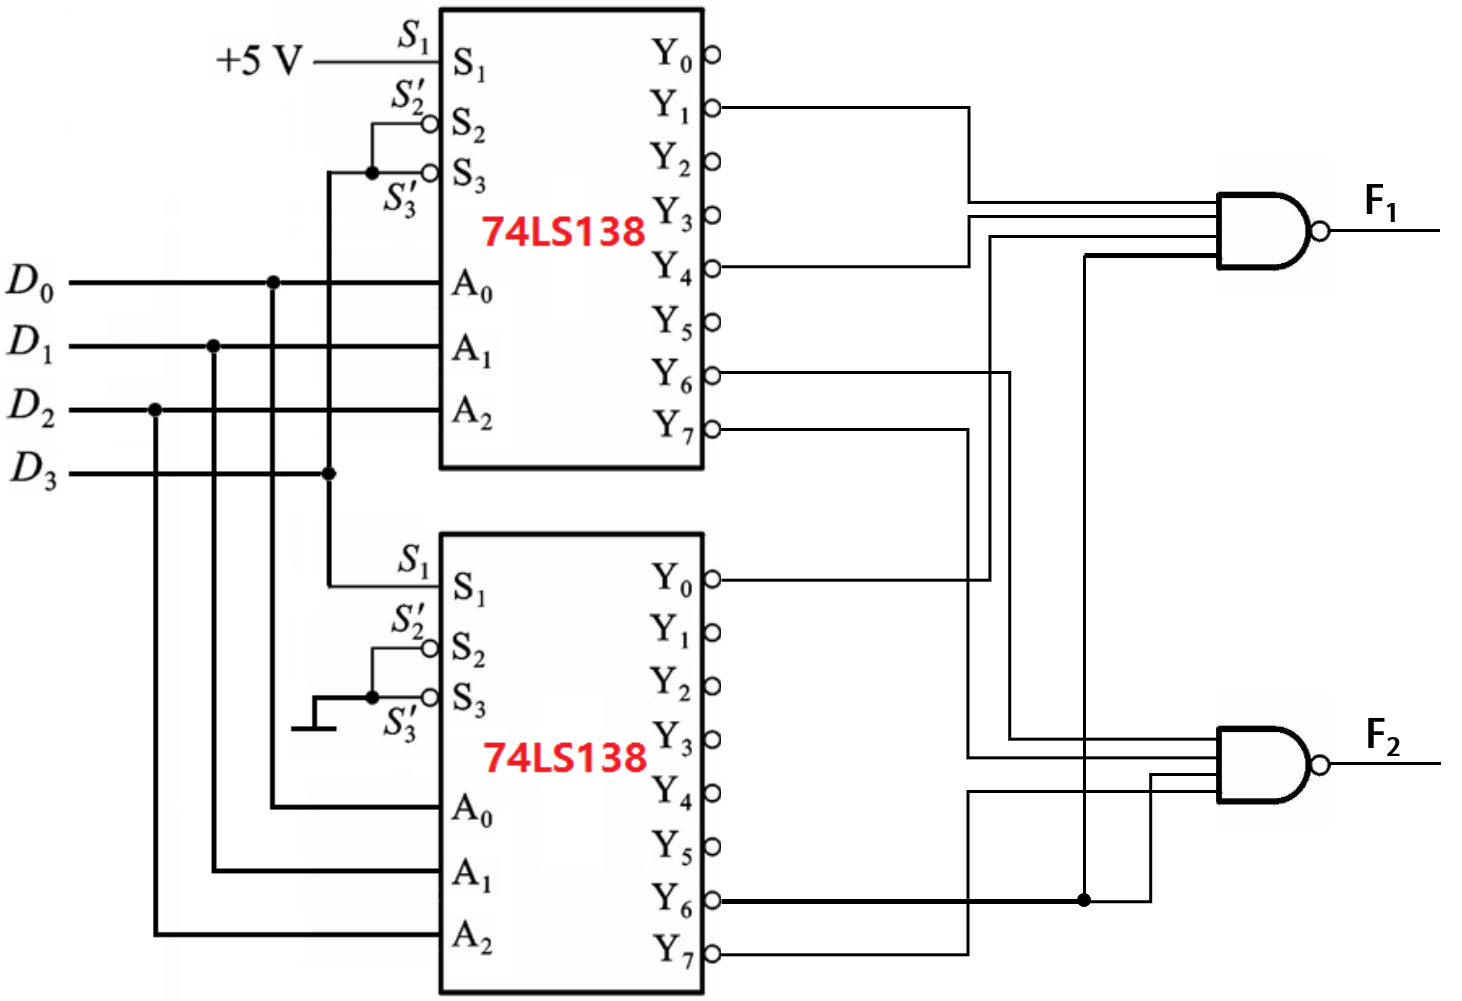
\includegraphics[width=0.5\linewidth]{pb1.png}}
  \caption{思考题一电路图}
  \label{fig:pb1}
  \end{figure}

\end{document}
